\section{League of Legends - Liga Diamante}

O \textit{League of Legends} tem vindo a se apresentar como uma nova tendência que atrai cada vez mais jovens, o seu crescimento exponencial levou à criação de uma modalidade de \textit{esports} que desde então tem somado atração pública. Ao longo dos últimos anos, em 2479 torneios, foram atribuídos perto de 80 milhões de dólares em prémios, sendo que o campeonato mundial de 2018 arrecadou um prémio de cerca de 6 milhões de dólares.

Como tal, facilmente conseguimos perceber que o interesse neste tipo de modalidades já não é o simples entretenimento, e que existem quantidade avultadas de dinheiro a ser movidas, o que implica que qualquer análise mais aprofundada aos comportamentos do jogo podem vir a ser lucrativos.

Então, pretendemos tentar modelar os efeitos que os primeiros minutos de jogo podem ter sobre o resultado final de forma a perceber os fatores decisivos numa partida.

% STEP 2 IN CRISP DM METODOLY
\subsection{Compreensão dos Dados}
Para estes dados utilizamos recursos disponíveis na internet\footnote{\url{https://www.kaggle.com/bobbyscience/league-of-legends-diamond-ranked-games-10-min}} e descobrimos um dataset que fornece, de forma sucinta, dados sobre os 10 primeiros minutos das duas equipas (azul e vermelha) utilizando um universo amostral de 10000 membros de uma das ligas mais elevadas do jogo, estes dados incidem exaustivamente sobre todas as metas no jogo como, por exemplo,

\begin{itemize}
    \item Ouro total recolhido, para cada equipa.
    \item Número de execuções, para cada equipa.
    \item Número de wards colocadas, para cada equipa.
\end{itemize}

No total, existem 19 atributos distintos para cada uma das equipa, o que perfaz um total de 38 atributos. Utilizando conhecimento de domínio facilmente conseguimos perceber que ter o mesmo atributo para cada uma das equipas não é indicativo, pelo que seria ideal conseguir agregar ambas as equipas em atributos idênticos.

É também importante denotar que, por conhecimento de domínio, existem atributos que estão necessariamente correlacionados. Por exemplo, o número de execuções da equipa azul e o número de mortes da equipa vermelha estão fortemente correlacionados negativamente, como seria de esperar.

% STEP 3 IN CRISP DM METODOLOGY
\subsection{Preparação dos Dados}
A nível de preparação de dados pouco foi feito, no entanto é importante denotar os seguintes aspectos chaves, que foram cruciais na nossa investigação.

\begin{itemize}
    \item A atributo \texttt{gameID} é completamente irrelevante pois é uma chave única associada a cada jogo, sem nenhum tipo de relevància física, por isso esse atributo foi removido.
    \item Os atributos \texttt{blueWins} e \texttt{redWins} são ambos binários e disjuntos, o que significa que a soma será sempre 1, pois numa dada partida apenas uma equipa pode ganhar. Como tal, consideramos apenas o atributo \texttt{blueWins}, tornando o problema num de prever a vitória ou derrota desta mesma equipa.
    \item De igual forma, os atributos \texttt{blueFirstBlood} e \texttt{redFirstBlood} seguem a mesma condição, pelo que só vale a pena ponderar um destes atributos.
    \item Nos restantes atributos, considerar tanto os atributos da equipa azul e vermelha não faz sentido. Na verdade, estamos interessados em perceber qual a diferença entre os resultados obtidos pela equipa azul num dado atributo e aqueles obtidos pela equipa vermelha. Assim sendo, os restantes atributos, 36, foram reduzidos a 18 por via de \textit{feature engineering}, sendo que no final os atributos em si passam a representar a diferença entre as 2 equipas.
\end{itemize}

Com isto em mente, podemos agora analisar as correlações existentes de forma mais compreensível.

\begin{figure}[H]
    \centering
    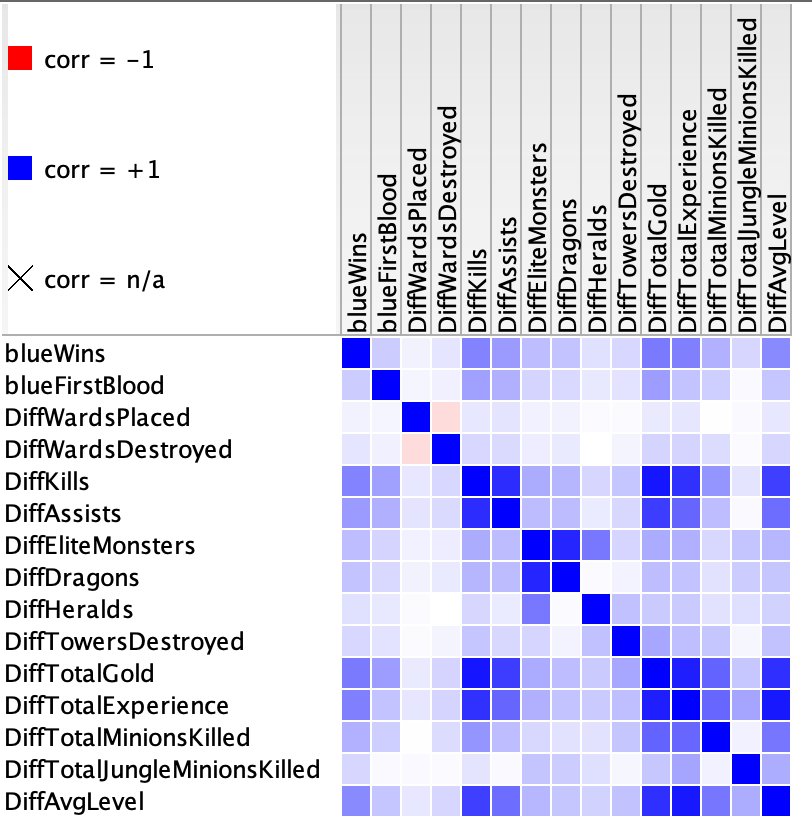
\includegraphics[width=0.5\linewidth]{Figures/RankCorrelation.png}
    \caption{Correlação entre features após processamento.}
    \label{fig:corr1}
\end{figure}

Pela figura \ref{fig:corr1} conseguimos detetar algumas correlações menos óbvios do que obtidas anteriormente. Por exemplo, podemos observar que a diferença em kills está fortemente correlacionada positivamente à diferença em ouro entre as duas equipas.

\begin{figure}[H]
    \centering
    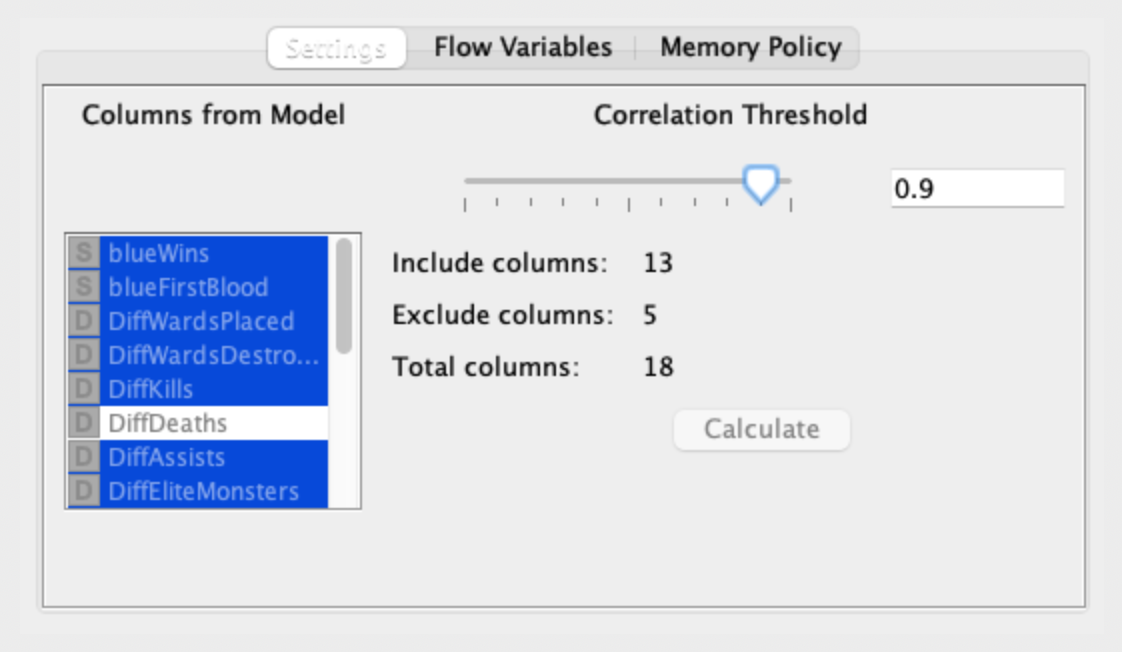
\includegraphics[width=0.5\linewidth]{Figures/Screenshot_2020-11-25_at_22.10.32.png}
    \caption{Seleção automática de features correlacionadas.}
    \label{fig:corr2}
\end{figure}


Como é desnecessário considerar atributos fortemente correlacionados entre si, utilizamos um correlation filter com as configurações da figura \ref{fig:corr2}.

% STEP 4 IN CRISP DM METODOLOGY
\subsection{Modelação}
De forma a garantir a ausência de overfitting decidimos que o ideal seria considerar um modelo baseado em \textit{random forest} que, devido à sua aleatoriadade, permite reduzir fortemente o overfitting.

Com métodos auxiliares de hyper-parameter tuning, fomos capazes de descobrir os hyper-parâmetros ideias para o nosso problema e re-aplicar esses parâmetros directamente na previsão do nosso test set, obtendo uma accuracy perto de 73\%, como se verifica em capítulos adiante. 

% STEP 5 IN CRISP DM METODOLOGY
\subsection{Apreciação dos Modelos}
Utilizando \textit{cross validation} com 10 \textit{folds}, foi possível chegar à conclusão de que a \textit{accuracy} do nosso modelo tende a rondar os 92\% que é, de longe, muito melhores que os nossos modelos iniciais, onde a \textit{accuracy} rondava sempre os 88-89\%. Como tal, este modelo foi seleccionado para ser submetido.